\documentclass[12pt]{article}

\title{Advanced Research Computing Coursework Report}
\author{James Hughes}

\usepackage[hidelinks]{hyperref}
\usepackage{url}
\usepackage{color}
\usepackage{listings}
\usepackage{graphicx}
\usepackage{subcaption}
\usepackage[export]{adjustbox}
\def\UrlBreaks{\do\/\do-}
\definecolor{codegreen}{rgb}{0, 0.6, 0}
\definecolor{codegray}{rgb}{0.9, 0.9, 0.9}

\lstdefinestyle{style1}{
    language=C++,
    basicstyle=\ttfamily\footnotesize,
    keywordstyle=\color{blue},
    backgroundcolor=\color{codegray},
    breakatwhitespace=false,
    breaklines=true,
    captionpos=b,
    commentstyle=\color{codegreen},
    keepspaces=true,
    numbers=left,
    numbersep=5pt,
    showspaces=false,
    showstringspaces=false,
    showtabs=false,
    tabsize=2
}
\lstset{style=style1}

\begin{document}

\maketitle

\newpage

\tableofcontents

\newpage

\section*{Introduction}

Conway's Game of Life first made an appearance in public discourse in 1970,
when Martin Gardner wrote a brief article introducing the concept in his column Mathematical Games in Scientific American\cite{gameoflife}.
The piece briefly describes game, stating its rules,
and displaying various diagrams of interesting simple behaviours such as periodicity and indefinite movement across the board.
It is notable that Gardner starts by suggesting that readers use `counters and a board', or failing that, `pencil and graph paper',
to see a demonstration of the game in action.
This is in stark contrast to the situation today, where plenty of computer simulations are easily accesible online \cite{playgameoflife},
enabling the game's interesting behaviours at scale to be easily explored.
This project seeks to take the ease of implementing this simulation with modern computing tools a step further,
by treating it as an exercise in developing highly optimised and parallelised code,
with a focus on maximising the performance of the simulation algorithm when run at scale.

The Game of Life consists of a large orthogonal grid of cells which exist in either one of two states: `dead' or `alive'.
At each stage or `tick' of the simulation, the state of each cell is updated according to its own current state,
and the current state of the cells adjacent (including diagonally) to it.
The only state changes occur when:

\begin{itemize}
    \item an `alive' cell fewer than two or more than three `alive' neighbours will become `dead' in the next tick, and
    \item a `dead' cell with exactly three `alive' neighbours will become `alive' in the next tick \cite{gameoflife}.
\end{itemize}

The evolution of the state of any cell within the simulation is thus bound by a deterministic rule that only depends on the current state of the simulation in a localised area.
This makes it akin to physical simulations of the real-world, for instance discrete numerical techniques to solve PDEs that relate to fluid dynamics.
In this sense, it is a suitable choice of problem to demonstrate the role of high-performance computing at the frontier of scientific research.

While the focus of this project was to produce highly optimised code,
care was taken to balance this with traditional best practices in software development.
The general approach in the first instance was to create code that was readable and verified via unit tests,
and only once this stage was reached was the code then iteratively re-factored to be increasingly optimised.
This ensured that the maintainability and robustness of the earlier code could be preserved as much as possible,
despite the tendency of optimisation to reduce these qualities.
In summary, the strategy of development sought primarily to demonstrate sophisticated optimisation techniques,
while not losing sight of computer scientist Donald Knuth's sage advice \cite{10.1145/356635.356640}:

\begin{quote}
    ``Premature optimization is the root of all evil.''
\end{quote}

\section*{Algorithm Design and Early Development}

The simulation primarily consists of a large orthogonal grid of cells, each of which changes state over time.
Therefore the first consideration in carrying out this simulation computationally was the abstraction and storage of this grid in memory.
Conceptually, operations need to occur at two levels of abstraction:
\begin{itemize}
    \item the level of matrix operations, including reading the state (stored in binary) of a cell and counting the number of alive neighbours; and
    \item the level of simulation operations, such as evolving the simulation, storing how many ticks have passed, and displaying the result.
\end{itemize}

Therefore, both a \texttt{Matrix} and a \texttt{World} class were created to store methods and attributes relevant to these respective levels.
\texttt{World} objects store two \texttt{Matrix} objects as members, to represent the current state of the simulation, and the next state.
The higher-level \texttt{World} objects also store an \texttt{age} attribute to keep track of the progress of the simulation,
and whose parity determines which of the two grids stores the current state.
The \texttt{Matrix} class stores, among others, a \texttt{count\_neighbours} method,
the first prototype of which is shown below:

\begin{lstlisting}
Matrix matrix::count_neighbours(Matrix A) {
    Matrix B = Matrix(A.n_rows - 2, A.n_cols - 2);

    for (int i = 1; i < A.n_rows - 1; i++) {
        for (int j = 1; j < A.n_cols - 1; j++) {
            for (int p = -1; p < 2; p++) {
                for (int q = -1; q < 2; q++) {
                    B(i - 1, j - 1) += A(i + p, j + q);
                }
            }
            B(i - 1, j - 1) -= A(i, j);
        }
        std::cout << std::endl;
    }
    return B;
}
\end{lstlisting}

This routine iterates across all of the entries of A (besides the edges) and then across all neighbours of said entry,
summing all of the values to return the results in matrix B - which is easy to understand and debug.
Similarly, the first prototype for the routine used to update cells according to the rules was written in an intuitive way:

\begin{lstlisting}
int conway::evaluate_rules(Matrix cells_count, Matrix &cells_current,
    Matrix &cells_next) {
    for (int i = 1; i < cells_count.n_rows - 1; i++) {
        for (int j = 1; j < cells_count.n_cols - 1; j++) {
            if (cells_current(i, j) == 1) {
                if (cells_count(i, j) != 2 and cells_count(i, j) != 3) {
                    cells_next(i, j) = 0;
                } else {
                    cells_next(i, j) = 1;
                }
            } else {
                if (cells_count(i, j) == 3) {
                    cells_next(i, j) = 1;
                } else {
                    cells_next(i, j) = 0;
                }
            }
        }
    }
}
\end{lstlisting}

The routine evaluates a set of nested if statements,
which first inspects the current state of the cell, and then checks the counts of the neighbouring cells accordingly.
Both of these fundamental routines were kept separate from the handling of the periodic boundary.
Within the \texttt{World} class, the grid of cells was represented as a matrix that had an extra row of cells on each edge.
There was then a separate routine to handle the update of these edges to implement a periodic boundary,
by copying each `proper' edge and vertex of the grid to the corresponding opposite `extra' edge or vertex.
Therefore the evolution of the simulation by one tick is decomposed into updating this boundary first, and then updating the cells.

This modular quality of the code enabled precise verification early on in the project,
and indeed developing a suite of unit tests via GoogleTest was the next step after prototyping.
This ensured that these core routines behaved as expected, and handled edge cases, forming part of a testing led-development strategy.
Creating the test suite involved the anticipation of other important functions that handled the input and output of matrices, for instance.
This ensured that the later development was more efficient as the modular organisation of the code, and the role of each routine, had already been planned out.
Moreover, the modularity contributed to a more maintanable code, particularly with the separate handling of the boundary,
in that different styles of boundaries (such as constant or reflective padding) could be easily implemented later on.
This was incidentally beneficial in the later stages of optimisation where these routines could be easily incorporated with the communication of halos during domain decomposition.

\section*{Optimisation and Parallelisation}

Optimisation was first achieved by single-thread improvements.
The focus was on the fundamental simulation routines since the performance of these becomes increasingly important as the scale of the simulation increases.
A major improvement in this respect was changing the \texttt{count\_neighbours} method to exploit the separability of the box blur convolution \cite{sepfilter},
in the following fashion:

\begin{lstlisting}
Matrix matrix::count_neighbours(Matrix &A) {
    int n_rows = A.n_rows;
    int n_cols = A.n_cols;

    // Row convolution
    Matrix B(n_rows, n_cols);
    for (int i = 0; i < n_rows; i++) {
        for (int j = 1; j < n_cols - 1; j++) {
            B(i, j) = A(i, j - 1) + A(i, j) + A(i, j + 1);
        }
    }

    // Column convolution
    Matrix C(n_rows, n_cols);
    for (int i = 1; i < n_rows - 1; i++) {
        for (int j = 1; j < n_cols - 1; j++) {
            C(i, j) = B(i - 1, j) + B(i, j) + B(i + 1, j);
        }
    }
    return C;
}
\end{lstlisting}

Note that in addition to the separation of the convolution into two one-dimensional kernels, the routine now includes the target cell entry in the count,
thereby removing the need to subtract this value in line 17.
This reduces the number of operations to compute each count from 10 in the earlier prototype to 6.
Additionally, the first row convolution has the extra benefit of accessing both matrices A and B contiguously,
since all entries of A accessed in each iteration lie in the same row of the matrix.

\begin{table}[hp]
    \centering
    {\footnotesize
    \begin{tabular}{| c | c | c |}
        \hline
        Matrix size & Prototype time (ms) & Separable convolution (ms) \\
        \hline
        2    & 0.0000658   &    0.0001272  \\
        3    & 0.003598    &    0.0001808  \\
        4    & 0.0097835   &    0.0004059  \\
        \hline
        6    & 0.0160791   &    0.0001572  \\
        7    & 0.0210006   &    0.0002301  \\
        8    & 0.0255929   &    0.0002429  \\
        \hline
        14   & 0.0476087   &    0.0004165  \\
        15   & 0.039723    &    0.0007573  \\
        16   & 0.0394387   &    0.0008217  \\
        \hline
        30   & 0.134101    &    0.0005995  \\
        31   & 0.115235    &    0.0007182  \\
        32   & 0.0972259   &    0.0013144  \\
        \hline
        62   & 0.431404    &    0.0018366  \\
        63   & 0.326085    &    0.0020772  \\
        64   & 0.325566    &    0.0038449  \\
        \hline
        126  & 1.48509     &    0.0319895  \\
        127  & 0.925173    &    0.0282965  \\
        128  & 1.32786     &    0.0354224  \\
        \hline
        254  & 5.63889     &    0.185919   \\
        255  & 6.37235     &    0.197116   \\
        256  & 6.23367     &    0.171525   \\
        \hline
        510  & 19.1519     &    0.538269   \\
        511  & 20.3742     &    0.602934   \\
        512  & 22.1763     &    0.760738   \\
        \hline
        1022 & 63.7401     &    2.37999    \\
        1023 & 67.6161     &    3.1337     \\
        1024 & 59.022      &    3.58696    \\
        \hline
        2046 & 165.155     &    9.53187    \\
        2047 & 172.047     &    9.17258    \\
        2048 & 202.097     &    12.758     \\
        \hline
        4094 & 608.048     &    53.6286    \\
        4095 & 554.764     &    66.2772    \\
        4096 & 580.508     &    70.9785    \\
        \hline
        8190 & 1949.4      &    242.911    \\
        8191 & 2085.35     &    249.298    \\
        8192 & 1959.89     &    289.589    \\
        \hline

    \end{tabular}
    }
    \caption{Mean of 10 timed runs on square matrices, comparing two implementations of \texttt{count\_neighbours}}.
    \label{tab:sepconvtime}
\end{table}


The performance gain was documented by the \texttt{time\_count\_neighbours} script, the results of which are found in Table \ref{tab:sepconvtime}.
For the largest matrices in the table this optimisation has the effect of a speed up of roughly 8-fold,
which increases even further for smaller matrices.
It should also be noted that there appears to be a cache-resonance effect for matrices of size larger than 500,
significant slow-downs for sizes that are powers of two beyond this number (512, 1024 and so on.).
In later timing scripts therefore, these sizes of simulation are avoided, so as not to confound different performance factors.

Incorporating a transposition of matrix \texttt{B} was also experimented with, both by including a standalone loop to compute a separate matrix \texttt{B\_T},
as well as computing \texttt{B\_T} directly from \texttt{A} instead of \texttt{B}.
Theoretically this could enable both 1D convolutions to be computed as row convolutions,
such that they both benefit from contiguous array access.
However, this appeared to cause a decrease in performance.
This is also a reasonable outcome considering that both the convolution operations and the transposition involve $O(n^2)$ operations with respect to the matrix size $n$,
and so the gain from more efficient usage of the cache is offset by the extra number of total operations from the transposition itself, even at scale.
In this way, transposition is much more likely to be fruitful (at scale) in terms of performance in such a scenario if the main algorithm has a computational cost worse than $O(n^2)$.

The \texttt{evaluate\_rules} function was also optimised to produce the folowing code:

\begin{lstlisting}
int conway::evaluate_rules(Matrix &Cells_count, Matrix &Cells_current,
                           Matrix &Cells_next) {
    for (int i = 0; i < Cells_count.n_rows; i++) {
        for (int j = 0; j < Cells_count.n_cols; j++) {
            Cells_next(i, j) =
                (Cells_count(i, j) == 3) ||
                ((Cells_count(i, j) == 4) && (Cells_current(i, j) == 1));
        }
    }
    return 0;
}
\end{lstlisting}

The main improvement compared to the earlier versions of this function is that this routine has no if statements,
each of which can cause costly branch mis-predictions in the CP, a problem which scales with the size of the simulation.
This updated routine avoids the conditional control flow by employing a masking technique which exploits the binary nature of the cell states.
In fact, in this case the optimisation is arguably much quicker to intuit as someone reading the code for the first time;
it essentially updates each cell to alive only if there are two adjacent alive cells (in which case the cell could be alive or dead),
or if there are three and the cell is currently alive.
On a more subtle note, C++ implements short-circuit evaluation of these boolean operators,
meaning that the second expression evaluation can be bypassed when the first (true for or, false for and)
already determines the overall value of the boolean operator.
With this in mind, the more likely condition of `exactly 2 alive neighbours' is placed before `exactly 3 alive neighbours and current cell alive',
while the less likely condition of `exactly 3 alive neighbours' is placed before `current cell is alive',
with the aim of minimising the number of boolean expressions that must be evaluated.

The project explored the use of both MPI and OpenMP to make the code parallelised.
The main difference between the two interfaces is that unlike OpenMP, MPI `ranks' do not have access to a shared memory space,
instead having separate allocated memory that can be communicated across the ranks.
Therefore MPI was used to employ a domain decomposition of the simulation, that is,
dividing the simulation grid amongst the ranks to be separately evolved.
The main challenge with this is implementing an organised collective communication such that cells on the boundaries of each `chunk'
can be correctly updated with respect to the values of the correct neighbouring cells located on other ranks.

In the first instance this was done using a 1D topology, dividing the simulation along the vertical dimension.

\begin{figure}[hp]
    \begin{subfigure}{0.49\textwidth}
    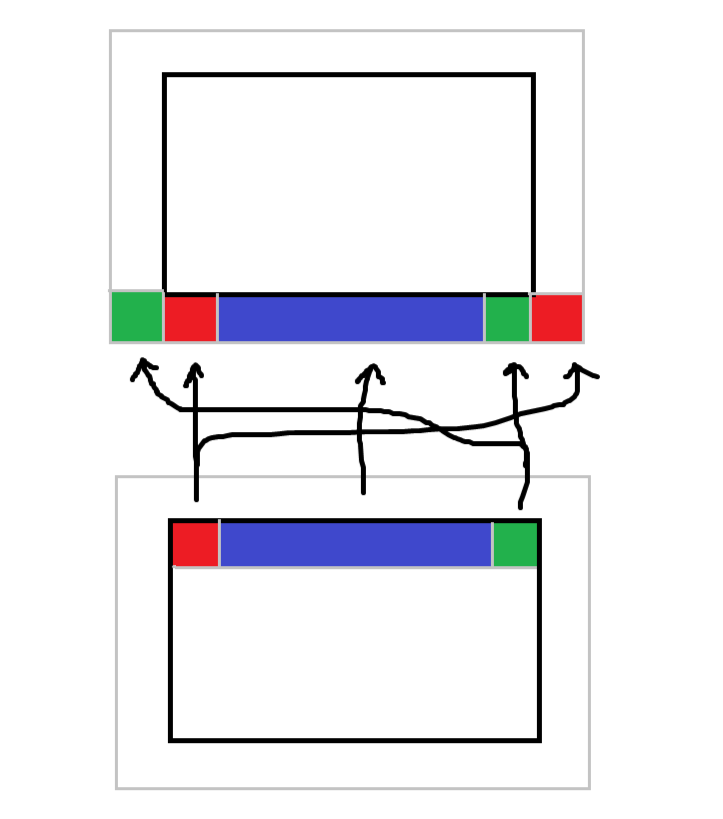
\includegraphics[width=0.9\linewidth, height=6cm, center]{figures/domain_decomp_1d_1.png}
    \caption{Required communication}
    \label{fig:domain_1d_1}
    \end{subfigure}
    \begin{subfigure}{0.49\textwidth}
    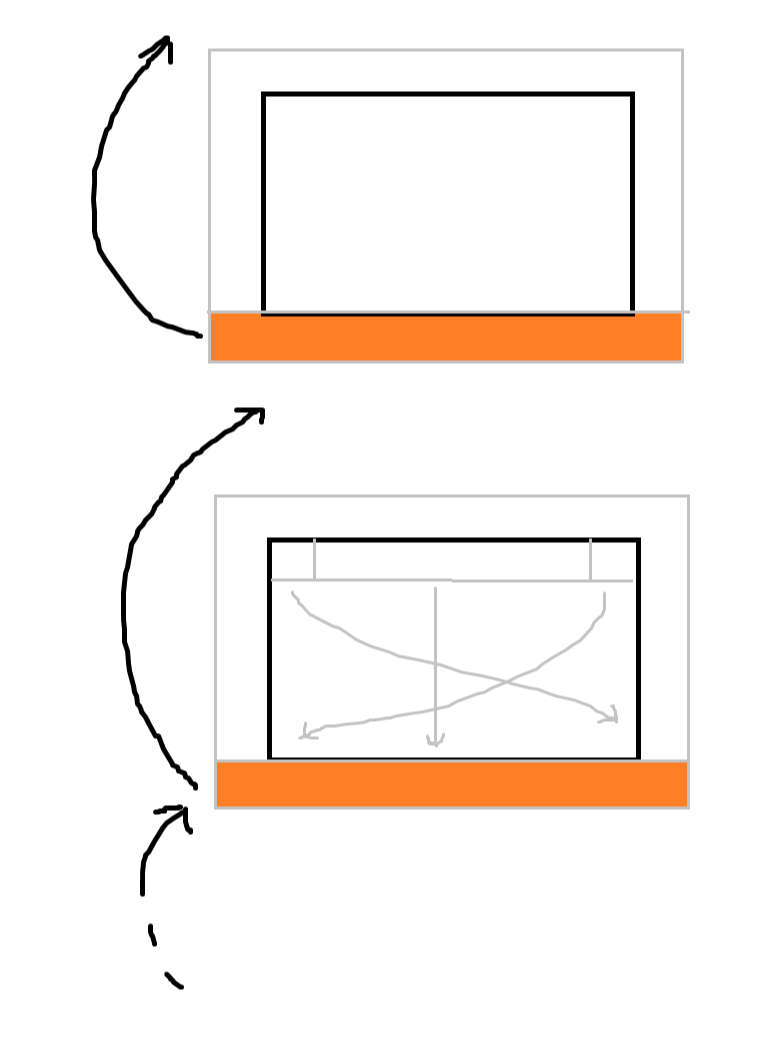
\includegraphics[width=0.9\linewidth, height=6cm, center]{figures/domain_decomp_1d_2.png}
    \caption{Two-step implementation}
    \label{fig:domain_1d_2}
    \end{subfigure}

    \caption{Illustration of the communication between chunks in 1D topology.}
    \label{fig:domain_1d}
\end{figure}

As previously mentioned, the pre-existing routine for updating the periodic boundary was helpful here.
This routine updates every `ghost' cell at the boundary of the matrix of cell values with the corresponding true inner cell value found on the opposite side of the matrix.
Without parallelisation this simply implements the periodic boundary at the extremes of the boundary.
But adding this as an extra step before communicating between ranks is also help, as shown in Figure \ref{fig:domain_1d}.
Without this step, vertices must be passed to multiple locations which can make it difficult to keep track of where cell values are communicated, as in Figure \ref{fig:domain_1d_1}.
Moreover, there must be separate communications for the edges and vertices.

On the other hand, Figure \ref{fig:domain_1d_2} demonstrates how using the intermediate update step makes the code more interpretable,
and thus maintainable and easier to debug (and develop into the 2D topology).
In this method, the communication can be done in just two MPI statements:

\begin{lstlisting}
// Cycle edges
MPI_Sendrecv_replace(top_edge, N_COLS_TOTAL + 2, MPI_INT, rank_down, 42, rank_up, 42, MPI_COMM_WORLD, &status);
MPI_Sendrecv_replace(bottom_edge, N_COLS_TOTAL + 2, MPI_INT, rank_up, 42, rank_down, 42, MPI_COMM_WORLD, &status);
\end{lstlisting}

All ranks can store the top and bottom edge in buffers of the same name which are then simply cycled in the correct direction across adjacent ranks.

The approach for 2D domain decomposition was similar, with Figure \ref{fig:domain_2d} illustrating how this is made more elegant by updating each rank's halo first,
and then cycling the corresponding edges and vertices of all the halos.
The challenge for the 2D decomposition was to embed the ranks in a coordinate system such that each rank could communicate to its correct adjacent ranks,
but the two-step approach also made this more manageable.

\begin{figure}[hp]
    \begin{subfigure}{0.49\textwidth}
    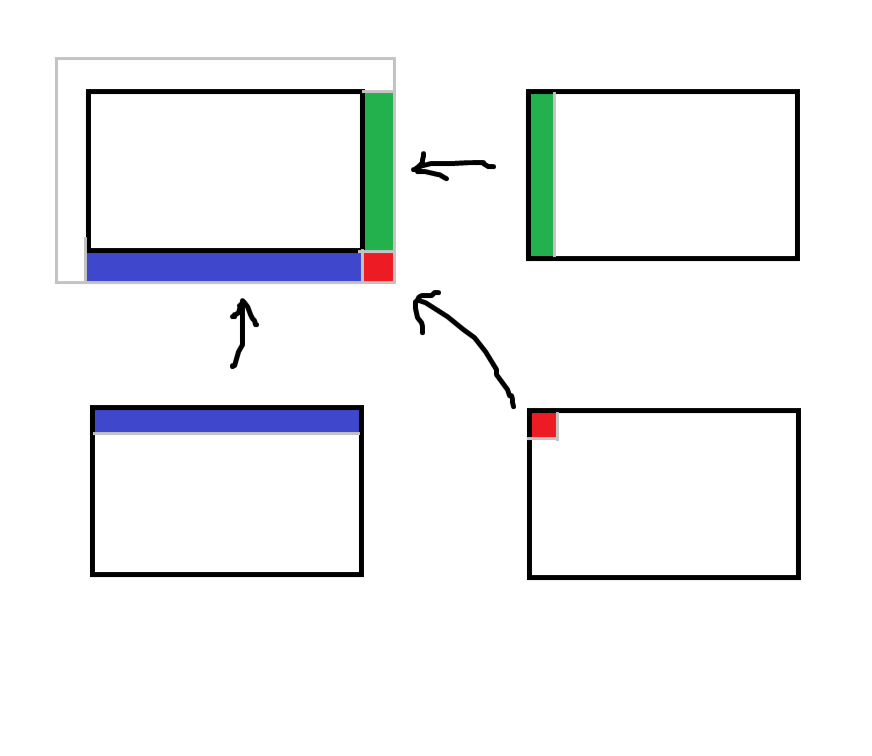
\includegraphics[width=0.9\linewidth, height=6cm, center]{figures/domain_decomp_2d_1.png}
    \caption{Required communication}
    \label{fig:domain_2d_1}
    \end{subfigure}
    \begin{subfigure}{0.49\textwidth}
    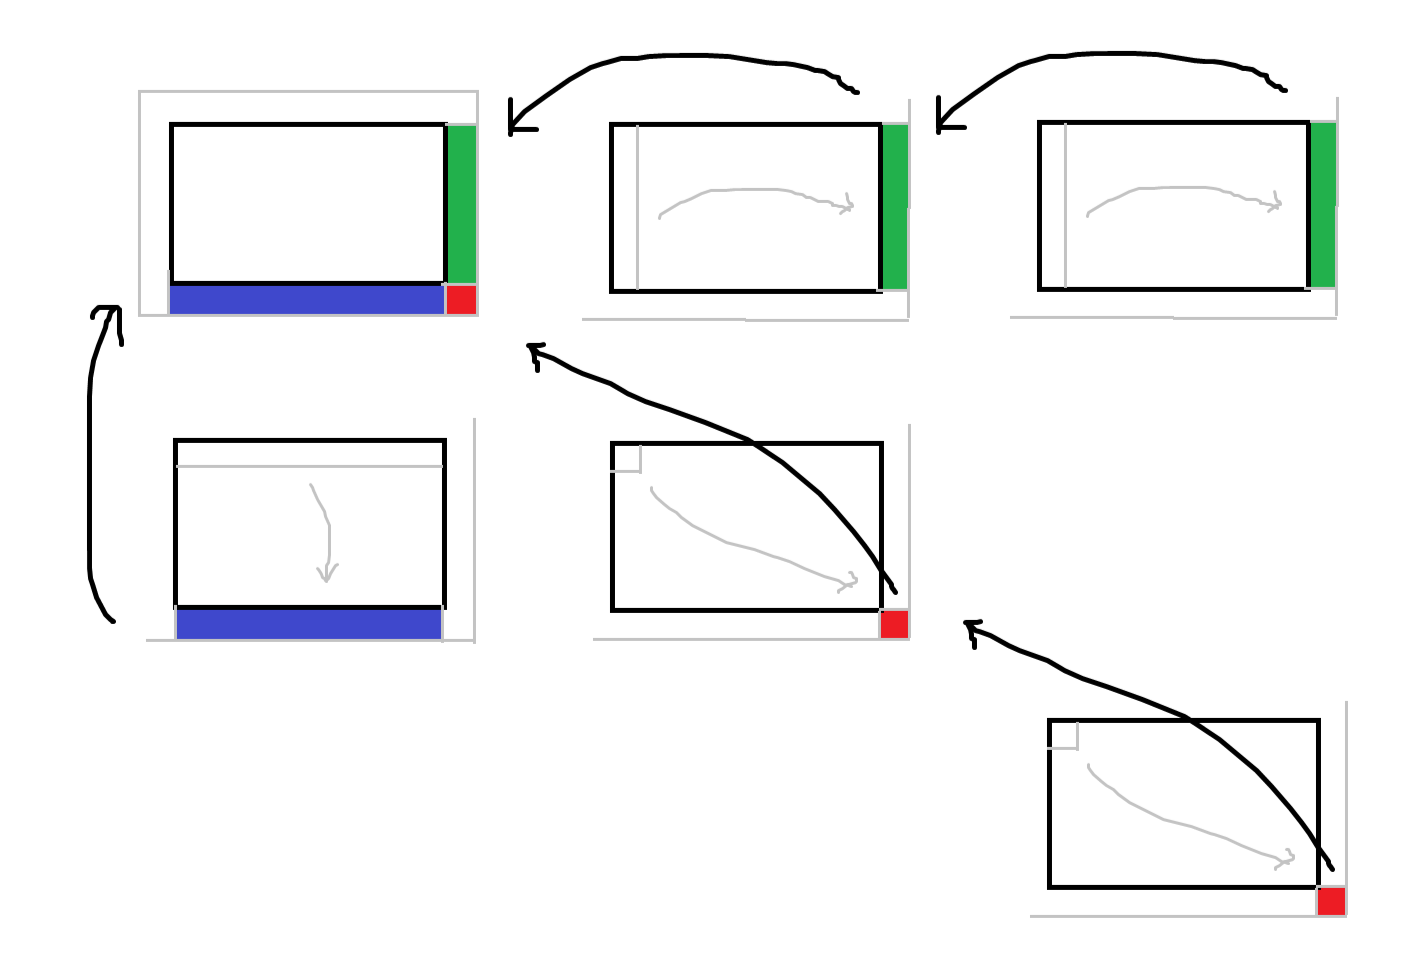
\includegraphics[width=0.9\linewidth, height=6cm, center]{figures/domain_decomp_2d_2.png}
    \caption{Two-step implementation}
    \label{fig:domain_2d_2}
    \end{subfigure}

    \caption{Illustration of the communication between chunks in 2D topology.}
    \label{fig:domain_2d}
\end{figure}

Once this worked for grids whose sizes were integer multiples of the topology sizes, it was extended to grids of any size.
This involves allocating differently sized chunks for the ranks.
In turn, if this is done properly then it does not affect the coherence communication of halos,
since corresponding halo edges will still always have the same size.
However, the scattering and gathering of the chunks at the start and end of the programme becomes more involved.
The sizes of each chunk are stored in a 2D array, and then the partial sums or `offsets' are computed from this,
which enables the use of the \texttt{MPI\_Scatterv} function to distribute across the differently sized buffers,
and the same calculations are passed to the \texttt{MPI\_Gatherv} function at the end.

The domain decomposition was then integrated with OpenMP functionality to employ threading within each rank.
This consisted of enabling the convolution, rule evaluation, and periodic boundary update to be performed by mutliple threads sharing the relevant array.
For this purpose, statements such as \texttt{\#pragma omp parallel for collapse(2)} were used to distribute the serial routines,
which mostly consisted of for loops, amongst the threads (with texttt{collapse(2)} implementing this for nested for loops).
Additionally, the setting of shared memory required the use of \texttt{\#pragma omp barrier} statements.
For instance, for the separable convolution algorithm, this was important because all entries of the intermediate row-convolved matrix are required to accurately perform the column convolution.
The barrier prevented idle threads from starting the column convolution iterations until the row convolution was complete.

\begin{figure}[hp]
    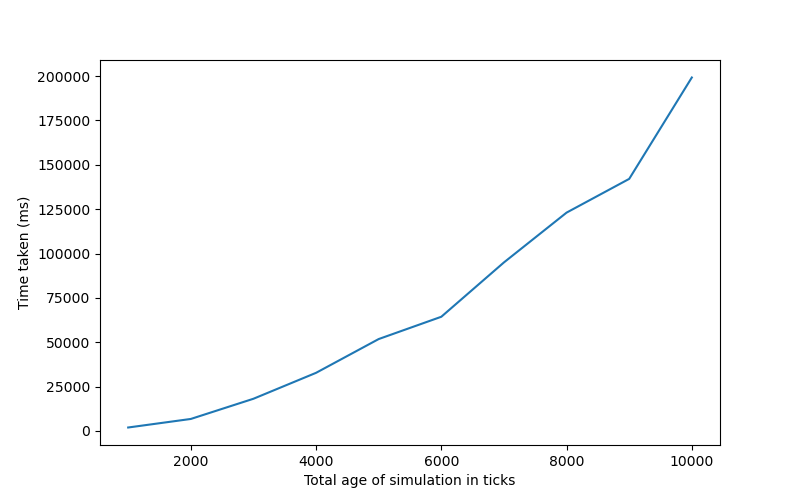
\includegraphics[scale=0.65, center]{figures/time_simulation.png}
    \caption{Timing plot for single thread code}
    \label{fig:time_r4}
\end{figure}

Once the hybrid parallel program was written and verified, it could be investigated via timing scripts and compared with the single-thread algorithm.



\begin{figure}[hp]
    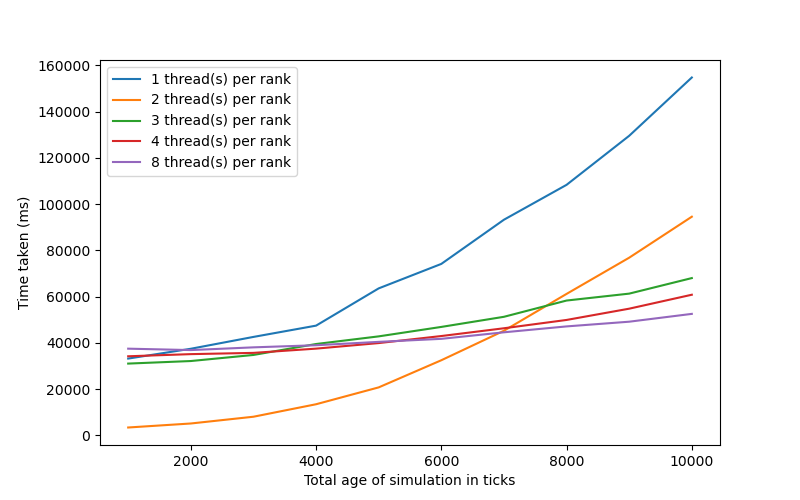
\includegraphics[scale=0.65, center]{figures/time_hybrid_r4_plot.png}
    \caption{Timing plot for 2x2 domain decomposition}
    \label{fig:time_r4}
\end{figure}

\begin{figure}[hp]
    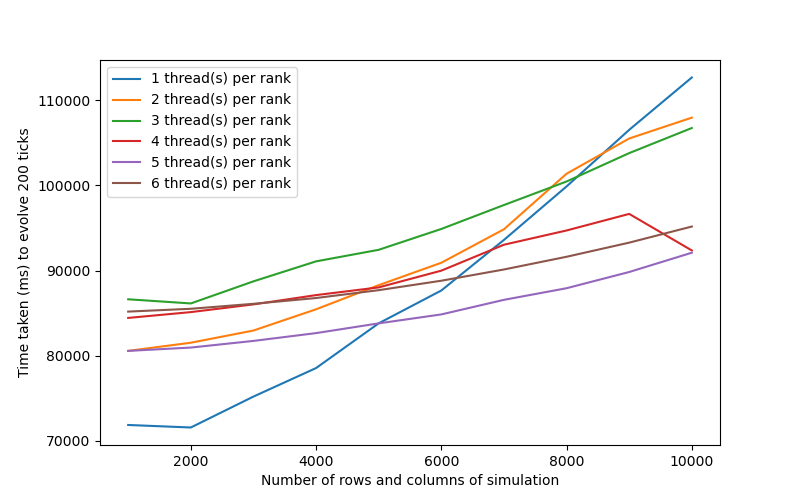
\includegraphics[scale=0.65, center]{figures/time_hybrid_r9_plot.png}
    \caption{Timing plot for 3x3 domain decomposition}
    \label{fig:time_r9}
\end{figure}

\begin{figure}[hp]
    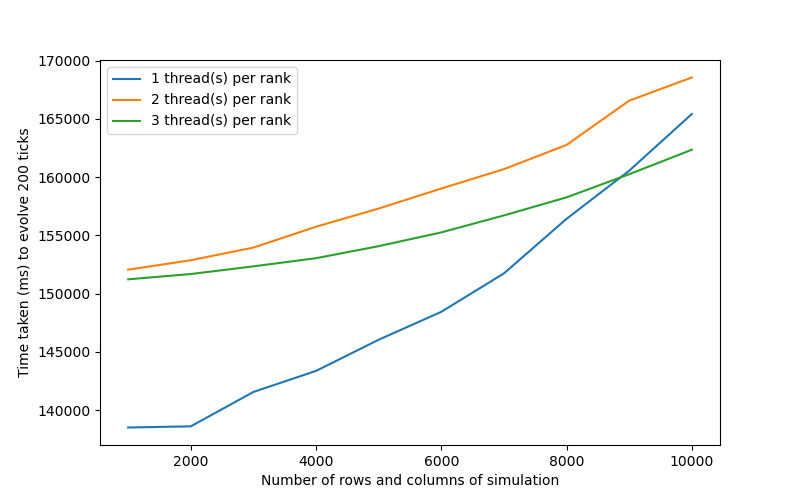
\includegraphics[scale=0.65, center]{figures/time_hybrid_r16_plot.png}
    \caption{Timing plot for 4x4 domain decomposition}
    \label{fig:time_r16}
\end{figure}

\begin{figure}[hp]
    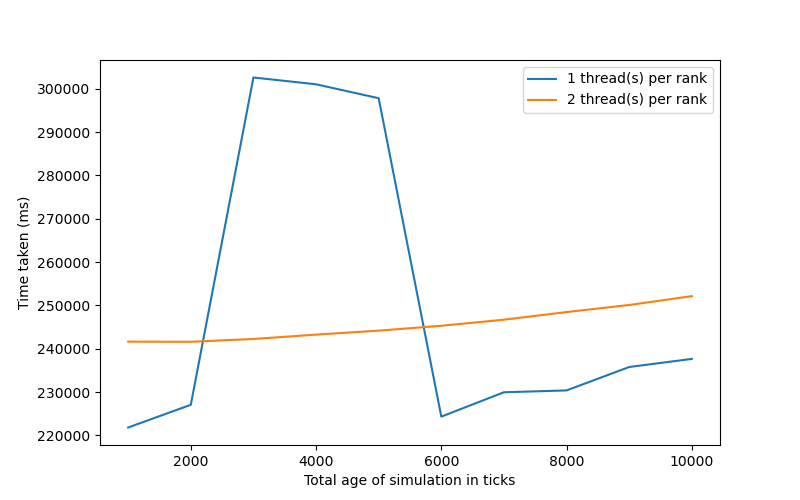
\includegraphics[scale=0.65, center]{figures/time_hybrid_r25_plot.png}
    \caption{Timing plot for 5x5 domain decomposition}
    \label{fig:time_r25}
\end{figure}

\begin{figure}[hp]
    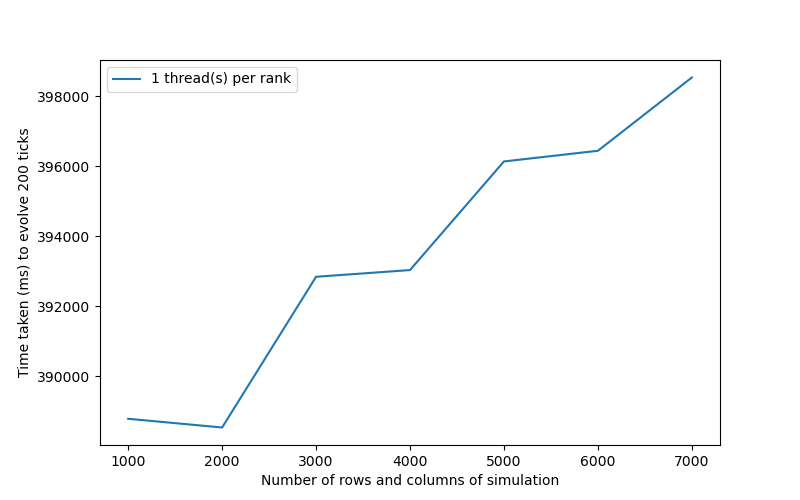
\includegraphics[scale=0.65, center]{figures/time_hybrid_r36_plot.png}
    \caption{Timing plot for 6x6 domain decomposition}
    \label{fig:time_r36}
\end{figure}

\begin{figure}[hp]
    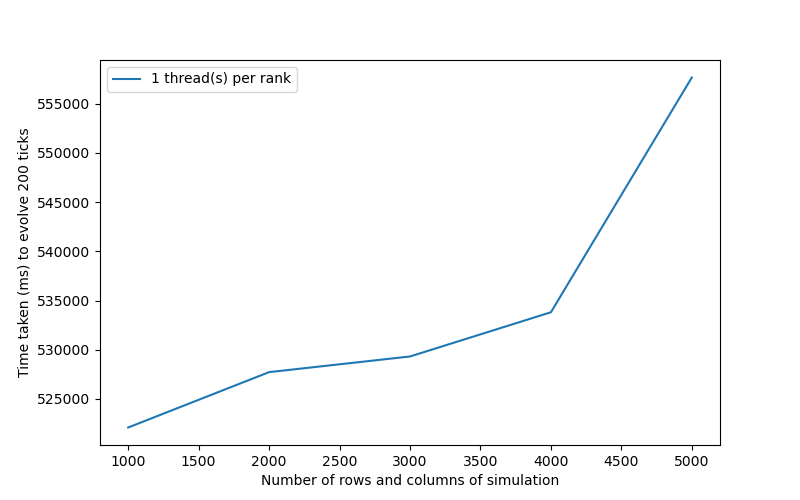
\includegraphics[scale=0.65, center]{figures/time_hybrid_r49_plot.png}
    \caption{Timing plot for 7x7 domain decomposition}
    \label{fig:time_r49}
\end{figure}


\section*{Summary}

Learnings: CSD3, C++, previous C1 things that were useful (e.g. versioning, branches)
What went to plan and what didn't:
How you could extend: refactoring of the code, niche things like avoiding cache resonance and automatically finding a topology; integrating 1d and 2d decomp.

\bibliographystyle{IEEEtran}
\bibliography{Biblio}

\appendix

\section{Statement on the use of auto-generation tools}

Auto-generation tools, such as GitHub or Microsoft Copilot, were not used at any stage during the development of the code within the repository of this project.
Similarly, none of the content of this report was produced -- or proofread -- by modern Large Language Models such as ChatGPT at any point.

\section {High-Performance Computing Resources}

This work was performed using resources provided by the Cambridge Service for Data Driven Discovery (CSD3) operated by the University of Cambridge Research Computing Service (www.csd3.cam.ac.uk),
provided by Dell EMC and Intel using Tier-2 funding from the Engineering and Physical Sciences Research Council (capital grant EP/T022159/1),
and DiRAC funding from the Science and Technology Facilities Council (www.dirac.ac.uk).

\end{document}
